% !TeX root = ../tfg.tex
% !TeX encoding = utf8

\chapter{Homología persistente}
\label{chapter:persistent-homology}

Este capítulo se dedica a la homología persistente, un concepto de gran
relevancia en la topología computacional que proporciona herramientas poderosas
para analizar y entender la estructura subyacente de los datos a través de
múltiples escalas. Originada en los trabajos iniciales de matemáticos como Edelsbrunner,
Letscher y Zomorodian \cite{edelsbrunner2002topological}, la homología persistente
permite la identificación y el análisis de características topológicas que persisten
a lo largo de variaciones en la escala en la que se observa.

Este capítulo se centrará en detallar los principios teóricos detrás de la homología
persistente. En particular, estudiaremos en profundidad el Teorema de correspondencia,
un resultado central en la teoría que muestra cómo transformar el nacimiento y
muerte de las clases de homología en objetos matemáticos más sencillos de
analizar y manipular computacionalmente. Seguiremos como esquema principal los resultados
de \cite{zomorodian2004computing} y \cite{dey2022computational}.

\section{Complejos de \u Cech y Vietoris-Rips}

La homología persistente es comúnmente empleada para analizar conjuntos de datos
representados como nubes de puntos. Aunque la homología en sí de estos conjuntos
puede no ser de gran interés debido a su simplicidad o falta de estructura topológica
relevante, la homología persistente permite revelar información de interés
mediante la construcción de estructuras topológicas construidas a partir de los
datos.

En este contexto, los complejos de \u Cech y Vietoris-Rips se emplean frecuentemente
para capturar la estructura topológica subyacente de las nubes de puntos. Estos
complejos dotan de estructura de complejo simplicial a los datos, facilitando su
representación, el estudio de su forma y sus características a múltiples escalas.

\begin{definicion}
	Sea $X$ un espacio topológico y sea $\mathcal{U}= \{U_{v}\}_{v \in V}$ un recubrimiento
	de $X$ por puntos $v \in V$. Llamaremos \textbf{nervio} de $\mathcal{U}$ al complejo
	simplicial abstracto con conjunto de vértices $V$ tal que la familia $v_{0}, \dots
	, v_{p} \in V$ genera un $p$-símplice si, y sólo si, $U_{v_0}\cap \dots \cap U_{v_p}
	\neq \emptyset$. Lo notaremos por $N(\mathcal{U})$.
\end{definicion}

\begin{definicion}
	Sea $(X,d)$ un espacio métrico y sea $V$ un subconjunto de puntos finito de $X$.
	Dado $\varepsilon > 0$, definimos el \textbf{complejo de \u Cech}
	$C(V, \varepsilon)$ como el nervio $N(\mathcal{B}_{\varepsilon})$, donde
	\[
	\mathcal{B}_{\varepsilon} = \{ B_{\varepsilon}(v) : v \in V \},
	\]
	siendo $B_{\varepsilon}(v)$ la bola abierta de centro $x$ y radio $\varepsilon
	> 0$.
\end{definicion}

\begin{proposicion}
	El complejo de \u Cech $C(V, \varepsilon)$ es un complejo simplicial abstracto.
\end{proposicion}
\begin{proof}
	Sea $V = \{v_{i}\}_{i=1}^{M}$ un subconjunto de puntos en el espacio métrico $X$.
	Fijado cierto $\varepsilon > 0$, definimos $\mathcal{B}_{\varepsilon} = \{B_{\varepsilon}
	(v) : v \in V \}$ como un recubrimiento por abiertos por puntos de $V$ del subespacio
	topológico $Y = \bigcup_{v \in V}B_{\varepsilon}(v)$. Veamos que el nervio
	$N(\mathcal{B}_{\varepsilon})$ de $\mathcal{B}_{\varepsilon}$ es el complejo
	abstracto cuyos vértices son los conjuntos $B_{\varepsilon}(x)$ y los
	símplices se forman por colecciones de estos conjuntos que tienen
	intersecciones no vacías.
	
	Supongamos que tenemos un símplice $\sigma = \{v_{i_1}, \ldots, v_{i_k}\}$ en
	$N(\mathcal{B}_{\varepsilon})$. Esto implica que
	\[
	\bigcap_{j=1}^{k} B_{\varepsilon}(v_{i_j}) \neq \emptyset.
	\]
	Consideremos ahora cualquier subconjunto de bolas de la forma $\{B_{\varepsilon}
	(v_{i_j})\}_{j \in J}$ donde $J \subseteq \{1, \ldots, k\}$. Es claro que por
	ser $\sigma$ un símplice,
	\[
	\bigcap_{j \in \{1, \ldots, k\} \setminus J}B_{\varepsilon}(v_{i_j}) \neq \emptyset
	,
	\]
	por lo que el conjunto de vértices restantes también forma un símplice en $N(\mathcal{B}
	_{\varepsilon})$. Por lo tanto, todas las caras de cualquier símplice $\sigma$
	son también símplices en $N(\mathcal{B}_{\varepsilon})$. Es decir, el nervio $N
	(\mathcal{B}_{\varepsilon})$ es cerrado bajo inclusiones.
	
	Dado que $V$ es finito y cada símplice se define como un subconjunto de $V$,
	entonces cada símplice sólo puede tener un número finito de subconjuntos. En consecuencia,
	el número de caras de cada símplice también es finito.
\end{proof}

El siguiente teorema será de utilidad para comprender y estudiar el espacio topológico
que definen los complejos de \u Cech. Por motivos de espacio, no trataremos la prueba
y simplemente enunciaremos el resultado. Una demostración del teorema enunciado
de forma más general puede encontrarse en \cite{hatcher2002algebraic}.

\begin{teorema}
	[Teorema del nervio] \label{teo:nerve} Sea $X$ un espacio métrico y sea $\mathcal{U}
	= \{U_{v}\}_{v \in V}$ un recubrimiento por abiertos finito de $X$. Supongamos
	además que para todo subconjunto no vacío de vértices $S \subseteq V$ tenemos
	que $\bigcap_{s \in S}U_{s}$ es contráctil o vacío. Entonces, el politopo de
	la realización geométrica del nervio de $\mathcal{U}$, $|N(\mathcal{U})|$, es
	homotópicamente equivalente a $X$.
\end{teorema}

Claramente, la intersección de bolas abiertas es vacía o contráctil (pues es convexa).
Por el \nameref{teo:nerve}, tenemos que el poliedro de la realización geométrica
del complejo de \u Cech es homotópicamente equivalente al subespacio métrico formado
por la unión de dichas bolas. En consecuencia, el estudio de la topología del complejo
de \u Cech se resume al estudio de las bolas que recubren sus vértices. Sin
embargo, el complejo de \u Cech es costoso de obtener mediante métodos computacionales.
Por ello, se propone el complejo de Vietoris-Rips para resolver este problema.

\begin{definicion}
	Sea $(X,d)$ un espacio métrico y sea $V$ un subconjunto de puntos de $X$. Dado
	$\varepsilon > 0$, definimos el \textbf{complejo de Vietoris-Rips}
	$VR(V,\varepsilon)$ como el complejo abstracto cuyo conjunto de vértices es
	$V$, de forma que $\{v_{0}, v_{1}, \dots v_{p}\} \subseteq V$ genera un $p$-símplice
	si, y solo si, $d(v_{i},v_{j}) \leq \varepsilon$ para todo $0 \leq i$,
	$j \leq p$.
\end{definicion}

\begin{proposicion}
	El complejo de Vietoris-Rips $VR(V,\varepsilon)$ es un complejo simplicial abstracto.
\end{proposicion}

\begin{proof}
	Primero veamos que el conjunto es cerrado bajo inclusiones. Supongamos que
	$\sigma = \{v_{0}, v_{1}, \dots, v_{p}\}$ es un $p$-símplice en
	$VR(V, \varepsilon)$. Por definición, esto significa que para todo $i, j$ tal
	que $0 \leq i, j \leq p$, se cumple que $d(v_{i}, v_{j}) \leq \varepsilon$.
	Consideremos ahora un subconjunto no vacío
	$\tau = \{v_{i_1}, v_{i_2}, \dots, v_{i_k}\} \subseteq \sigma$. Para cualquier
	par de índices $a, b$ con $1 \leq a, b \leq k$, los vértices $v_{i_a}$ y
	$v_{i_b}$ también cumplen que $d(v_{i_a}, v_{i_b}) \leq \varepsilon$, pues $\tau
	\subseteq \sigma$. Por lo tanto, $\tau$ es un $(k-1)$-símplice en $VR(V, \varepsilon
	)$.
	
	Por otro lado, cada $p$-símplice $\sigma$ en $VR(V, \varepsilon)$ es un
	subconjunto finito de $V$. El número de subconjuntos de cualquier conjunto finito
	es finito, y en particular, el número de subconjuntos de $\sigma$ es $2^{|\sigma|}$,
	donde $|\sigma|$ es el número de vértices en $\sigma$. En consecuencia, cada
	símplice en $VR(V, \varepsilon)$ tiene un número finito de caras.
\end{proof}

\begin{figure}
	\centering
	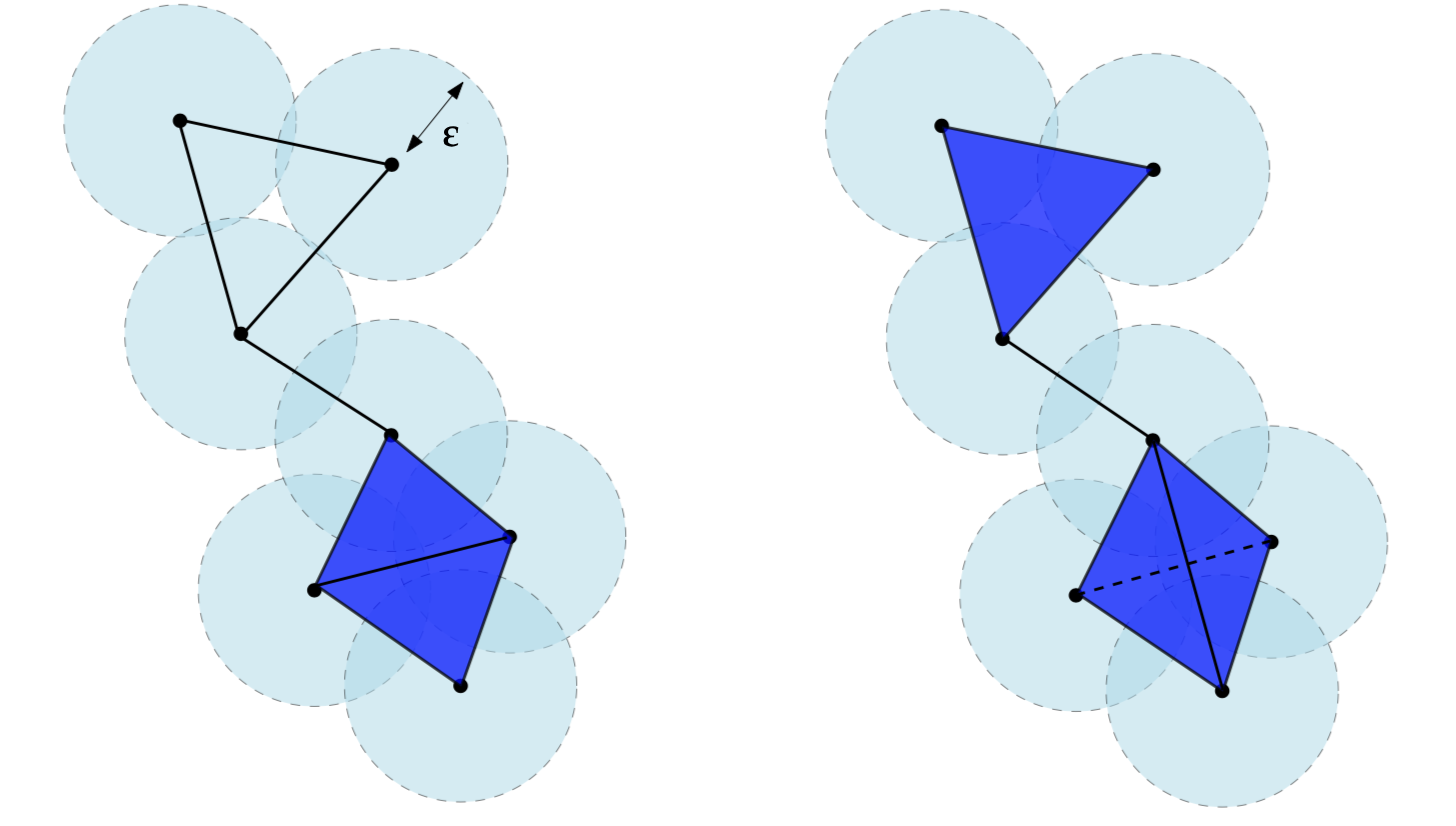
\includegraphics[width=110mm]{img/cech-vr.png}
	\caption{Representación de complejos simpliciales \u Cech (izquierda) y
		Vietoris-Rips (derecha) para un conjunto de puntos en $\mathbb{R}^{2}$. En el complejo
		de \u Cech, los símplices se forman por la intersección no vacía de círculos
		de radio $\varepsilon$ centrados en los puntos. El complejo de Vietoris-Rips conecta
		puntos que distan hasta $2\varepsilon$, independientemente de las
		intersecciones de los círculos. Los símplices de mayor dimensión están coloreados
		en azul, resaltando las diferencias en la estructura simplicial generada por
		cada método. Fuente \cite{chazal2021introduction}.}
\end{figure}

El complejo de Vietoris-Rips es interesante en el estudio de complejos de \u Cech.
Este hecho se debe a que estos últimos pueden ser aproximados en cierto sentido
por complejos de Vietoris-Rips:

\begin{proposicion}
	Sea $(X,d)$ un espacio métrico y sea $V$ un subconjunto de puntos de $X$.
	Entonces
	\[
	C(V, \varepsilon) \subseteq VR(V, 2\varepsilon) \subseteq C(V, 2\varepsilon).
	\]
\end{proposicion}
\begin{proof}
	La primera inclusión es inmediata pues si un punto $x$ pertenece a la intersección
	$\bigcap_{v \in V}B(v, \varepsilon)$, entonces la distancia para cada par de
	puntos de $V$ es, a lo sumo, $2 \varepsilon$. En consecuencia, cualquier
	símplice de $C(V,\varepsilon)$ se encuentra en $VR(V, 2\varepsilon)$.
	
	Para la segunda inclusión, consideremos ahora un símplice $\sigma = \{v_{0}, \dots
	, v_{p}\}$ de $VR(V, 2\varepsilon)$. Por la definición de complejo de Vietoris-Rips,
	tenemos que $d(v_{i}, v_{j}) \leq 2\varepsilon$ para todo $i,j \in \{0, \dots,
	p\}$. Considerando las bolas abiertas de radio $2\varepsilon$ centradas en
	$v_{i}$ y en $v_{j}$, tenemos que su intersección es no vacía, pues
	$v_{i} \in \overline{B}_{2\varepsilon}(v_{j})$ y
	$v_{j} \in \overline{B}_{2\varepsilon}(v_{i})$. En el supuesto de que los puntos
	pertenecieran a la frontera de las bolas, la intersección de las bolas
	abiertas también sería no vacía pues $\varepsilon > 0$. En consecuencia,
	tenemos que $\sigma \in C(V,2\varepsilon)$.
\end{proof}

\section{Módulos de homología persistente}

El módulo de homología persistente es el objeto central de estudio en este
capítulo. A partir de filtraciones de complejos simpliciales, esta estructura
nos va a permitir realizar un estudio de la homología simplicial de dicha
filtración.

\begin{definicion}
	Sea $K$ un complejo simplicial. Una \textbf{filtración} $\mathcal{F}$ de $K$ es
	una familia totalmente ordenada de subcomplejos $\{K^{n}\}_{n \in \N}$ tal que
	$\emptyset, K \in \mathcal{F}$ y si $i \leq j$, entonces
	$K^{i} \subseteq K^{j}$. En particular, llamaremos a dicho orden \textbf{filtro}.
\end{definicion}
A partir de la definición anterior, podemos construir los complejos de cadenas asociados
$C(K^{i};R)$ para todo $i \in \N$. Así mismo, podemos obtener sus respectivos submódulos
de ciclos $Z_{p}(K^{i})$ y bordes $B_{p}(K^{i})$ para cada $R$-módulo de cadenas
orientadas $C_{p}(K^{i};R)$.
\begin{definicion}
	Sea $\mathcal{F}$ una filtración, sea $p$ un número natural y sean
	$i,j \in \{0, \dots, n\}$ tales que $i \leq j$. Definimos el \textbf{$(i,j)$-ésimo
		$R$-módulo de homología persistente de dimensión $p$} asociado a $\mathcal{F}$
	como
	\[
	H_{p}^{i \to j}(\mathcal{F};R) := \im f_{p}^{i \to j},
	\]
	donde $f_{p}^{i \to j}$ es el homomorfismo inducido entre las clases de
	homología de la inclusión que va de $K^{i}$ a $K^{j}$. El rango de $H_{p}^{i
		\to j}(\mathcal{F};R)$ diremos que es el \textbf{$(i,j)$-ésimo número de Betti
		de persistencia de dimensión $p$} y lo notaremos por $\beta_{p}^{i \to j}$.
\end{definicion}
\begin{proposicion}
	Sea $\mathcal{F}$ una filtración del complejo simplicial $K$. Entonces
	\[
	H_{p}^{i \to j}(\mathcal{F};R) \cong \frac{Z_{p}(K^{i})}{B_{p}(K^{j}) \cap Z_{p}(K^{i})}
	\]
	es un isomorfismo de $R$-módulos.
\end{proposicion}
\begin{proof}
	Sabemos que el cociente anterior está bien definido, pues
	$Z_{p}(K^{i}) \cap B_{p}(K^{j})$ es un submódulo de $Z_{p}(K^{i})$. Para ver que
	en efecto existe un isomorfismo, consideraremos la proyección
	$\pi_{i} : Z_{p}(K^{i}) \to H_{p}(K^{j};R)$. Aplicando el \nameref{teo:first-iso},
	tenemos que
	\[
	\frac{Z_{p}(K^{i})}{\ker \pi_{i}}\cong \im \pi_{i}
	\]
	es un isomorfismo. Sin embargo, nótese que
	\begin{align*}
		\ker \pi_{i} & = \{z \in Z_{p}(K^{i}) : \pi_{i}(z) = [0] \} = \{z \in Z_{p}(K^{i}) : [z] = [0] \} \\
		& = \{z \in Z_{p}(K^{i}) : z \in B_{p}(K^{j}) \} = B_{p}(K^{j}) \cap Z_{p}(K^{i}).
	\end{align*}
	Además,
	\begin{align*}
		H_{p}^{i \to j}(\mathcal{F};R) & = \im f_{p}^{i \to j}= \{f_{p}^{i \to j}([z]) : [z] \in H_{p}(K^{i};R) \}                                  \\
		& = \{[({i_{i,j}}_{*})_{p}(z)] : z \in Z_{p}(K^{i}) \} = \{\pi_{i}(z) : z \in Z_{p}(K^{i}) \} = \im \pi_{i}.
	\end{align*}
\end{proof}
%
%\tikzset{every picture/.style={line width=0.75pt}} %set default line width to 0.75pt
%
%\begin{tikzpicture}[x=0.75pt,y=0.75pt,yscale=-1,xscale=1]
%	%uncomment if require: \path (0,235); %set diagram left start at 0, and has height of 235
%
%	%Shape: Ellipse [id:dp28793519162441483]
%	\draw  [fill={rgb, 255:red, 74; green, 144; blue, 226 }  ,fill opacity=1 ] (81,72.52) .. controls (81,21.96) and (104.41,-19.03) .. (133.29,-19.03) .. controls (162.18,-19.03) and (185.59,21.96) .. (185.59,72.52) .. controls (185.59,123.08) and (162.18,164.07) .. (133.29,164.07) .. controls (104.41,164.07) and (81,123.08) .. (81,72.52) -- cycle ;
%	%Shape: Ellipse [id:dp5681689316325549]
%	\draw  [fill={rgb, 255:red, 169; green, 208; blue, 255 }  ,fill opacity=1 ] (213.98,71.12) .. controls (213.98,20.55) and (237.39,-20.44) .. (266.27,-20.44) .. controls (295.15,-20.44) and (318.56,20.55) .. (318.56,71.12) .. controls (318.56,121.68) and (295.15,162.67) .. (266.27,162.67) .. controls (237.39,162.67) and (213.98,121.68) .. (213.98,71.12) -- cycle ;
%	%Shape: Ellipse [id:dp8309047921029127]
%	\draw  [fill={rgb, 255:red, 169; green, 208; blue, 255 }  ,fill opacity=1 ] (349.94,72.52) .. controls (349.94,21.96) and (373.35,-19.03) .. (402.24,-19.03) .. controls (431.12,-19.03) and (454.53,21.96) .. (454.53,72.52) .. controls (454.53,123.08) and (431.12,164.07) .. (402.24,164.07) .. controls (373.35,164.07) and (349.94,123.08) .. (349.94,72.52) -- cycle ;
%	%Shape: Ellipse [id:dp6471754723664047]
%	\draw  [fill={rgb, 255:red, 169; green, 208; blue, 255 }  ,fill opacity=1 ] (484.41,72.52) .. controls (484.41,21.96) and (507.82,-19.03) .. (536.71,-19.03) .. controls (565.59,-19.03) and (589,21.96) .. (589,72.52) .. controls (589,123.08) and (565.59,164.07) .. (536.71,164.07) .. controls (507.82,164.07) and (484.41,123.08) .. (484.41,72.52) -- cycle ;
%	%Shape: Ellipse [id:dp2887350161913229]
%	\draw  [fill={rgb, 255:red, 74; green, 144; blue, 226 }  ,fill opacity=1 ] (226.68,99.38) .. controls (226.68,64.42) and (244.4,36.09) .. (266.27,36.09) .. controls (288.14,36.09) and (305.86,64.42) .. (305.86,99.38) .. controls (305.86,134.33) and (288.14,162.67) .. (266.27,162.67) .. controls (244.4,162.67) and (226.68,134.33) .. (226.68,99.38) -- cycle ;
%	%Shape: Ellipse [id:dp5997979826300346]
%	\draw  [fill={rgb, 255:red, 74; green, 144; blue, 226 }  ,fill opacity=1 ] (362.64,100.78) .. controls (362.64,65.83) and (380.37,37.49) .. (402.24,37.49) .. controls (424.1,37.49) and (441.83,65.83) .. (441.83,100.78) .. controls (441.83,135.73) and (424.1,164.07) .. (402.24,164.07) .. controls (380.37,164.07) and (362.64,135.73) .. (362.64,100.78) -- cycle ;
%	%Shape: Ellipse [id:dp7175957985808079]
%	\draw  [fill={rgb, 255:red, 74; green, 144; blue, 226 }  ,fill opacity=1 ] (505.7,114.81) .. controls (505.7,87.61) and (519.58,65.55) .. (536.71,65.55) .. controls (553.83,65.55) and (567.71,87.61) .. (567.71,114.81) .. controls (567.71,142.02) and (553.83,164.07) .. (536.71,164.07) .. controls (519.58,164.07) and (505.7,142.02) .. (505.7,114.81) -- cycle ;
%	%Straight Lines [id:da9382562350971808]
%	\draw    (133.29,-19.03) -- (266.27,36.09) ;
%	%Straight Lines [id:da8538877694649378]
%	\draw    (266.27,36.09) -- (402.24,37.49) ;
%	%Straight Lines [id:da415521229926751]
%	\draw    (402.24,37.49) -- (536.71,65.55) ;
%	%Straight Lines [id:da5906511807851325]
%	\draw [fill={rgb, 255:red, 74; green, 144; blue, 226 }  ,fill opacity=1 ] [dash pattern={on 0.84pt off 2.51pt}]  (266.27,16.65) -- (399.25,16.65) ;
%	%Straight Lines [id:da7445210416359846]
%	\draw  [dash pattern={on 0.84pt off 2.51pt}]  (399.25,16.65) -- (536.71,114.81) ;
%
%	% Text Node
%	\draw (260.27,-0.47) node [anchor=north west][inner sep=0.75pt]    {\(\alpha \)};
%	% Text Node
%	\draw (375.75,-4.04) node [anchor=north west][inner sep=0.75pt]    {\(f_{p}^{i,j-1}( \alpha )\)};
%	% Text Node
%	\draw (515.12,113.56) node [anchor=north west][inner sep=0.75pt]    {\(f_{p}^{i,j}( \alpha )\)};
%	% Text Node
%	\draw (100.29,-38.98) node [anchor=north west][inner sep=0.75pt]    {\(H_{p}( K_{i-1})\)};
%	% Text Node
%	\draw (242.52,-40.98) node [anchor=north west][inner sep=0.75pt]    {\(H_{p}( K_{i})\)};
%	% Text Node
%	\draw (370.99,-39.38) node [anchor=north west][inner sep=0.75pt]    {\(H_{p}( K_{j-1})\)};
%	% Text Node
%	\draw (510.2,-39.98) node [anchor=north west][inner sep=0.75pt]    {\(H_{p}( K_{j})\)};
%	% Text Node
%	\draw (260,12.4) node [anchor=north west][inner sep=0.75pt]    {\(\bullet \)};
%	% Text Node
%	\draw (393,12.4) node [anchor=north west][inner sep=0.75pt]    {\(\bullet \)};
%	% Text Node
%	\draw (528,108.4) node [anchor=north west][inner sep=0.75pt]    {\(\bullet \)};
%\end{tikzpicture}

La homología persistente facilita la interpretación de la homología en los distintos
niveles de la filtración, permitiendo un análisis cuantitativo de su evolución. Al
observar el nacimiento y desaparición de las clases de homología mediante los módulos
de homología persistente, se obtiene información detallada de la estructura
topológica general de la filtración.

\begin{figure}[h]
	\centering
	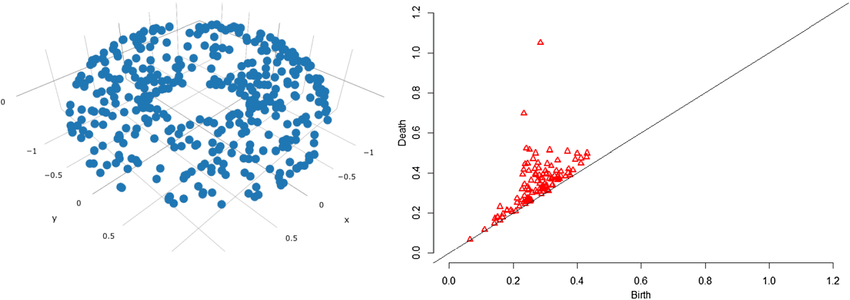
\includegraphics[width=\textwidth]{img/persistence-diagram.png}
	\caption{Diagrama de persistencia para la homología de dimensión 1 de la
		filtración de Vietoris-Rips de 2000 puntos i.i.d. en un toro. El gráfico
		destaca dos puntos significativos que representan las clases de equivalencia
		de los ciclos unidimensionales del toro, destacando su persistencia topológica.
		Fuente \cite{divol2019}.}
\end{figure}

\begin{definicion}
	Dada una filtración $\mathcal{F}$, decimos que un elemento $\alpha \neq 0$ en
	$H_{p}(K^{i};R)$ \textbf{nace} en $K^{i}$ si $\alpha \not\in H_{p}^{i-1 \to i}(
	\mathcal{F};R)$. Además, decimos que $\alpha$ \textbf{muere} en $K^{j}$ si se
	fusiona con una clase proveniente de una dimensión anterior cuando se desplaza
	de $K^{j-1}$ a $K^{j}$. Esto es, si
	$f^{i \to j-1}_{p}(\alpha) \not\in H_{p}^{i-1 \to j-1}(\mathcal{F};R)$ pero
	$f^{i \to j}_{p}(\alpha) \in H_{p}^{i-1 \to j}(\mathcal{F};R)$.
\end{definicion}

\begin{ejemplo}
	\label{ex:pers-homology} Consideremos un conjunto de vértices $\{0, e_{1}, e_{2}
	, e_{3}\} = V$ formado por los vectores de la base usual y el vector nulo en $\mathbb{R}
	^{3}$ con la topología usual. Definamos el complejo simplicial $K$ a partir
	del 2-símplice formado por dichos vectores y todas sus caras. A continuación,
	vamos a estudiar la filtración inducida por inclusiones $\mathcal{K}$:
	\[
	\emptyset = K^{0} \to K^{1} \to K^{2} \to K^{3} \to K^{4} = K,
	\]
	donde
	\begin{align*}
		K^{1} & = \{[0], [e_{1}], [e_{2}], [e_{3}]\},                                     \\
		K^{2} & = K^{1} \cup \{[0, e_{1}], [0, e_{2}], [0, e_{3}]\},                      \\
		K^{3} & = K^{2} \cup \{[0, e_{1}, e_{2}], [0, e_{1}, e_{3}], [0, e_{2}, e_{3}]\}.
	\end{align*}
	
	Consideremos además las cadenas de $\mathbb{R}$-módulos asociadas, donde cada $C
	_{p}(K^{j};\mathbb{R})$ es un espacio vectorial con cuerpo $\mathbb{R}$ para cada
	dimensión $p \in \mathbb{Z}$.
	
	En $K^{1}$, el módulo de cadenas $C_{0}(K^{1}; \mathbb{R})$ es generado por
	los 0-símplices $\{ [0], [e_{1}], [e_{2}], [e_{3}] \}$, lo que resulta en un espacio
	vectorial $\mathbb{R}^{4}$, mientras que los módulos
	$C_{1}(K^{1}; \mathbb{R})$ y $C_{2}(K^{1}; \mathbb{R})$ son ambos cero, debido
	a la ausencia de 1-símplices y 2-símplices.
	
	En cuanto a $K^{2}$, el módulo $C_{0}(K^{2}; \mathbb{R})$ conserva la misma
	estructura que $C_{0}(K^{1}; \mathbb{R})$, pues no se añaden nuevos 0-símplices.
	Sin embargo, $C_{1}(K^{2}; \mathbb{R})$ se genera ahora a partir de las aristas
	$\{ [0, e_{1}], [0, e_{2}], [0, e_{3}] \}$, formando un espacio vectorial
	isomorfo a $\mathbb{R}^{3}$. El módulo $C_{2}(K^{2}; \mathbb{R})$ sigue siendo
	nulo debido a la falta de 2-símplices.
	
	Llegando a $K^{3}$, observamos que $C_{2}(K^{3}; \mathbb{R})$ ahora se genera
	por $\{ [0, e_{1}, e_{2}], [0, e_{1}, e_{3}], [0, e_{2}, e_{3}] \}$, generando
	otro espacio isomorfo a $\mathbb{R}^{3}$. Los módulos
	$C_{0}(K^{3}; \mathbb{R})$ y $C_{1}(K^{3}; \mathbb{R})$ son idénticos a sus
	pares en $K^{2}$, pues tienen los mismos símplices de dimensión 1 y 2.
	
	Finalmente, en $K^{4} = K$, todos los módulos $C_{p}(K^{4}; \mathbb{R})$ para
	$p \in \{ 0, 1, 2 \}$ son idénticos a los de $K^{3}$. Sin embargo, $K^{4}$
	tiene un 3-símplice formado por todos sus vértices, de forma que $C_{3}(K^{4};
	\R) = \R$.
	
	En $K^{2}$, todos los 1-símplices son ciclos porque no existen 2-símplices que
	puedan generar bordes, de modo que $Z_{1}(K^{2}) = C_{1}(K^{2})$ y $B_{1}(K^{2}
	) = 0$. En $K^{3}$, todos los 2-símplices son ciclos, ya que no hay 3-símplices
	en esta etapa; así, $Z_{2}(K^{3}) = C_{2}(K^{3})$ y los bordes de
	$C_{1}(K^{3})$ son generados por las aristas de los 2-símplices, indicando cierta
	interacción entre ellos.
	
	En $K^{4}$, el único 3-símplice forma un ciclo por sí mismo, puesto que $C_{4}(
	K^{4}) = 0$ y, por lo tanto, $Z_{3}(K^{4}) = C_{3}(K^{4})$. Los bordes de los
	2-símplices en $C_{2}(K^{4})$ resultan de aplicar $\partial_{3}$ al 3-símplice,
	produciendo una combinación de todos los 2-símplices, por lo tanto, $B_{2}(K^{4}
	)$ se compone de estos bordes.
	
	Para $K^{1}$, tenemos $H_{0}(K^{1}; \R) = \mathbb{R}^{4}$, mostrando cuatro componentes
	conexas. En $K^{2}$, la homología se simplifica a $H_{0}(K^{2}; \R) = \mathbb{R}$,
	indicando que todos los vértices forman una única componente conexa, mientras que
	$H_{1}(K^{2}; \R) = 0$ y $H_{2}(K^{2}; \R) = 0$ dado que no hay 2-símplices.
	En $K^{3}$, la homología permanece sin cambios para $H_{0}$ y $H_{2}$, pero
	todos los posibles 1-ciclos se convierten en bordes de los 2-símplices, lo que
	resulta en $H_{1}(K^{3}; \R) = 0$.
	
	Finalmente, en $K^{4}$, observamos que $H_{0}(K^{4}; \R) = \mathbb{R}$,
	$H_{1}(K^{4}; \R) = 0$, $H_{2}(K^{4}; \R) = 0$ y $H_{3}(K^{4}; \R) = \mathbb{R}$,
	indicando la presencia de una cavidad tridimensional que no es el borde de
	ningún símplice de mayor dimensión.
	
	Tras este exhaustivo estudio de la homología de la filtración, por fin estamos
	en condiciones de estudiar el nacimiento o muerte de las clases de homología.
	Por ejemplo, podemos observar que en el instante 1 de la filtración nacen cuatro
	clases de homología de dimensión 0, pues $H_{0}(K^{1};\R) = \R^{4}$. Sin embargo,
	en el segundo instante de la filtración, $H_{0}(K^{2}; \R) = \R$, lo que
	implica la muerte de tres clases de homología de dimensión 0. De esta forma, tendríamos
	que el módulo de homología persistente $H_{0}^{1 \to 2}(\mathcal{K}; \R) = \im{i_*}
	^{1 \to 2}= \R$, siendo
	$i^{1 \to 2}_{*} : H_{0}(K^{1};\R) \to H_{0}(K^{2};\R)$ el homomorfismo de
	inclusión inducido. En consecuencia, es claro que $(1,2)$-ésimo número de
	Betti de persistencia de dimensión 0 es 1.
\end{ejemplo}

Como hemos visto en el \autoref{ex:pers-homology}, el estudio de la homología
persistente requiere de un amplio estudio de la homología de la filtración a
todos sus niveles. Esta información a menudo es numerosa y difícil de interpretar,
por lo que en la siguiente sección mostraremos una representación de la
homología persistente que facilite su estudio e interpretación.

\section{Representación de la homología persistente}
\label{sec:barcode}

Nuestro objetivo ahora es obtener una representación de la homología persistente
que nos permita interpretarla. Originalmente, esta representación se ha realizado
mediante los \textbf{diagramas de persistencia}. En estos diagramas, cada clase
de homología que nace en un complejo simplicial $K^{i}$ y muere en $K^{j}$ se
representa por un punto $(i, j)$ en el plano cartesiano, para cada dimensión $p$.

Aunque intuitivos, los diagramas de persistencia presentan ciertas limitaciones.
El principal problema radica en que no logran capturar de manera efectiva la multiplicidad
de la persistencia; es decir, múltiples clases que nacen y mueren simultáneamente
se representan mediante un mismo punto, lo que puede conducir a ambigüedades en
la interpretación de los datos.

Para abordar estos problemas, Zomorodian y Carlsson introdujeron un enfoque innovador
mediante el uso del \textbf{código de barras} \cite{zomorodian2004computing}. Este
método no solo ofrece una visualización clara y detallada de la vida de cada clase
de homología, sino que también facilita la interpretación de su multiplicidad y
relevancia en el contexto de los datos analizados. Esta interpretación fue posible
ya que demostraron que todo módulo de persistencia puede identificarse de manera
biyectiva con una estructura algebraica más general, conocida como \textbf{módulos
	graduados}, bajo ciertas hipótesis.

A continuación profundizaremos en la aplicación y las implicaciones de estos
métodos, explorando en detalle el Teorema de correspondencia como se discute en \cite{Corbet_2018}.

\begin{definicion}
	Sea $\mathcal{M}= \{\{M_{i}\}_{i \in \N}, \{f_{i,j}\}_{i \leq j \in \N}\}$ una
	familia de $R$-módulos. Diremos que dicha familia es un \textbf{módulo de
		persistencia discreto} sobre $R$ si para cada $i \leq j$ existe un homomorfismo
	de $R$-módulos $f_{i,j}: M_{i} \to M_{j}$ tal que:
	\begin{enumerate}
		\item El homomorfismo $f_{i} = f_{i,i}= \mathrm{id}_{M_i}$ para todo $i \in \mathbb{N}$.
		
		\item La composición $f_{i,k}\circ f_{i,j}= f_{i,k}$ para todo $i \leq j \leq
		k$.
	\end{enumerate}
\end{definicion}
\begin{observacion}
	Nótese que con esta definición, todo módulo de homología persistente es de
	hecho un módulo de persistencia discreto. Dada una dimensión $p \in \Z$ fija,
	los $R$-módulos los componen los módulos de homología y sus homomorfismos
	inducidos por la inclusión cumplen dichas propiedades.
\end{observacion}

\begin{definicion}
	Sean $\mathcal{M}= \{\{M_{i}\}_{i \in \N}, \{f_{i,j}\}_{i \leq j \in \N}\}, \mathcal{N}
	= \{\{N_{i}\}_{i \in \N}, \{g_{i,j}\}_{i \leq j \in \N}\}$ dos módulos de persistencia
	discretos. Diremos que la familia de homomorfismos
	$\varphi_{\bullet} = \{\varphi_{i}\}_{i \in \N}$ tales que
	$\varphi_{i} : M_{i} \to N_{i}$ es un \textbf{homomorfismo de módulos de
		persistencia discreto} si $g_{i,j}\circ \varphi_{i} = \varphi_{j} \circ f_{i,j}$.
\end{definicion}
La anterior definición es equivalente a decir que el diagrama
\[
\xymatrix{ M_0 \ar@{->}[r]^{f_0} \ar@{->}[d]^{\varphi_0} & M_1 \ar@{->}[r]^{f_1} \ar@{->}[d]^{\varphi_1} & \cdots \ar@{->}[r]^{f_{i-1}} & M_i \ar@{->}[r]^{f_i} \ar@{->}[d]^{\varphi_i} & M_{i+1} \ar@{->}[r]^{f_{i+1}} \ar@{->}[d]^{\varphi_{i+1}} & \cdots \\ N_0 \ar@{->}[r]^{g_0} & N_1 \ar@{->}[r]^{g_1} & \cdots \ar@{->}[r]^{g_{i-1}} & N_i \ar@{->}[r]^{g_i} & N_{i+1} \ar@{->}[r]^{g_{i+1}} & \cdots }
\]
conmuta. En las condiciones anteriores, los módulos de persistencia discretos
junto a sus homomorfismos forman una categoría que notaremos por $R$-$\Cat{PersMod}$.
Claramente se tiene que existe el homomorfismo identidad $\id_{\mathcal{M}}: \mathcal{M}
\to \mathcal{M}$, donde a cada módulo y homomorfismo de módulos se le asocia él
mismo. Además, la identidad conmuta con la familia de homomorfismos de módulos, pues
es la composición con la identidad de homomorfismos de módulos componente a componente.
Veamos ahora la asociatividad en la composición de los homomorfismos de módulos
de persistencia discretos. Consideremos cuatro módulos de persistencia discretos
$\mathcal{M}= \{\{M_{i}\}_{i \in \mathbb{N}}, \{f_{i,j}\}_{i \leq j \in
	\mathbb{N}}\}$,
$\mathcal{N}= \{\{N_{i}\}_{i \in \mathbb{N}}, \{g_{i,j}\}_{i \leq j \in
	\mathbb{N}}\}$, $\mathcal{P}= \{\{P_{i}\}_{i \in \mathbb{N}}, \{h_{i,j}\}_{i
	\leq j \in \mathbb{N}}\}$ y $\mathcal{Q}= \{\{Q_{i}\}_{i \in \mathbb{N}}, \{p_{i,j}
\}_{i leq j \in \mathbb{N}}\}$; y tres homomorfismos
$\varphi_{\bullet} : \mathcal{M}\to \mathcal{N}$, $\psi_{\bullet} : \mathcal{N}\to
\mathcal{P}$, y $\theta_{\bullet} : \mathcal{P}\to \mathcal{Q}$. Para demostrar la
asociatividad, necesitamos verificar que
\[
(\theta \circ (\psi \circ \varphi))_{i} = ((\theta \circ \psi) \circ \varphi)_{i}
\quad \forall i \in \mathbb{N}.
\]
Sin embargo, dicha composición es la asociatividad de la composición de homomorfismos
de módulos componente a componente, por lo que tenemos que:
\[
\theta_{i} \circ (\psi_{i} \circ \varphi_{i}) = (\theta_{i} \circ \psi_{i}) \circ
\varphi_{i}.
\]

Además, para cualquier $i \leq j$ en $\mathbb{N}$, necesitamos mostrar que:
\[
h_{i,j}\circ (\theta \circ (\psi \circ \varphi))_{i} = (\theta \circ (\psi \circ
\varphi))_{j} \circ f_{i,j}.
\]
Sustituyendo la definición de composición, esto se reduce a verificar que
\[
h_{i,j}\circ (\theta_{i} \circ (\psi_{i} \circ \varphi_{i})) = (\theta_{j} \circ
(\psi_{j} \circ \varphi_{j})) \circ f_{i,j}\quad i \leq j \text{ en }\N.
\]
O equivalentemente, que $((h_{i,j}\circ \theta_{i}) \circ \psi_{i}) \circ \varphi
_{i} = \theta_{j} \circ (\psi_{j} \circ (\varphi_{j} \circ f_{i,j}))$. Debido a
que cada homomorfismo respeta las estructuras de los módulos de persistencia, tenemos:
\[
h_{i,j}\circ \theta_{i} = \theta_{j} \circ p_{i,j},
\]
\[
p_{i,j}\circ \psi_{i} = \psi_{j} \circ g_{i,j},
\]
\[
g_{i,j}\circ \varphi_{i} = \varphi_{j} \circ f_{i,j}.
\]
Aplicando estas igualdades y la asociatividad de homomorfismos de módulos, concluimos
que:
\begin{align*}
	h_{i,j}\circ (\theta_{i} \circ (\psi_{i} \circ \varphi_{i})) & = ((h_{i,j}\circ \theta_{i}) \circ \psi_{i}) \circ \varphi_{i} = ((\theta_{j} \circ p_{i,j}) \circ \psi_{i}) \circ \varphi_{i}                                                                  \\
	& = (\theta_{j} \circ (p_{i,j}\circ \psi_{i})) \circ \varphi_{i} = (\theta_{j} \circ (\psi_{j} \circ g_{i,j})) \circ \varphi_{i}                                                                  \\
	& = \theta_{j} \circ ((\psi_{j} \circ g_{i,j}) \circ \varphi_{i}) = \theta_{j} \circ (\psi_{j} \circ (g_{i,j}\circ \varphi_{i})) = \theta_{j} \circ (\psi_{j} \circ (\varphi_{j} \circ f_{i,j})).
\end{align*}

\begin{definicion}
	Sea $R$ un anillo. Diremos que $R$ es un \textbf{anillo graduado} si puede descomponerse
	como una suma directa
	\[
	R = \bigoplus_{n=0}^{\infty}R_{n},
	\]
	donde $R_{m} R_{n} \subseteq R_{m+n}$ para todo $m, n \in \mathbb{Z}$, siendo
	el anillo $R_{m} R_{n} = \{ r_{m} r_{n} : r_{m} \in R_{m}, r_{n} \in R_{n} \}$.
	Los elementos de $R_{n}$ distintos de cero se denominan \textbf{homogéneos de
		grado $n$}.
\end{definicion}

\begin{definicion}
	Sea $R$ un anillo graduado y sea $M$ un $R$-módulo. Diremos que $M$ es un
	\textbf{módulo graduado} si puede escribirse como
	\[
	M = \bigoplus_{n=0}^{\infty}M_{n},
	\]
	donde $M_{n}$ son grupos abelianos y $R_{m} M_{n} \subseteq M_{m+n}$ para todo
	$m, n \in \mathbb{Z}$, siendo $R_{m} M_{n}$ el $R_{m}$-módulo con grupo
	abeliano $M_{n}$. Un elemento de $M_{n}$ distinto de cero se llama \textbf{homogéneo
		de grado $n$}.
\end{definicion}

Los módulos graduados no son más que un tipo particular de módulos. Para cada
módulo graduado $M$, el morfismo identidad $\mathrm{id}_{M} : M \to M$ es simplemente
el morfismo identidad de $R$-módulos. Este morfismo es claramente un
homomorfismo de módulos graduados que preserva la graduación. Consideremos ahora
dos módulos graduados $M$, $N$ y un homomorfismo de módulos graduados
$f: M \to N$. Si tenemos otro módulo graduado $P$ y un homomorfismo $g: N \to P$,
su composición $g \circ f$ es la composición de homomorfismos de $R$-módulos. Por
lo tanto, la asociatividad de la composición se sigue directamente de la
asociatividad de la composición de homomorfismos de $R$-módulos. En consecuencia,
los módulos graduados sobre $R$ junto con los homomorfismos de módulos graduados
forman una categoría, que denotaremos por $R\text{-}\mathbf{GrMod}$.

Los módulos de persistencia discretos sobre un anillo $R$ y los $R[t]$-módulos graduados
son conceptos íntimamente relacionados. Si $\mathcal{M}$ es un módulo de
persistencia discreto, podemos definir un $R[t]$-módulo graduado $\alpha(\mathcal{M}
)$ como
\[
\alpha(\mathcal{M}) = \bigoplus_{i \in \N}M_{i},
\]
donde el producto por $t$ lo definimos como $t \cdot m_{i} = f_{i,i+1}(m_{i})$ para
todo $m_{i} \in M_{i}$. Análogamente, podemos definir un módulo de persistencia discreto
a partir de un $R[t]$-módulo $\bigoplus_{i \in \N}M_{i}$, de forma que
\[
\beta \left( \bigoplus_{i \in \N}M_{i} \right) = \mathcal{M}.
\]
Aquí, los morfismos los obtenemos a partir del producto por $t$, esto es, $f_{i,
	i+1}(m_{i}) = t \cdot m_{i}$ para todo $m_{i} \in M_{i}$. El siguiente resultado
nos proporciona formalmente cómo de íntima es esta relación.

\begin{lema}
	\label{lem:repr-carlsson-no-finito} Las aplicaciones $\alpha$ y $\beta$ definidas
	anteriormente forman una pareja isomorfa de funtores covariantes entre $R$-$\Cat
	{PersMod}$ y $R[t]$-$\Cat{GrMod}$. En particular, ambas categorías son isomorfas.
\end{lema}
\begin{proof}
	Sea $\varphi_{\bullet} : \mathcal{M}\to \mathcal{N}$ un morfismo de módulos de
	persistencia discretos. Definamos
	\[
	\alpha(\varphi_{\bullet}) : \bigoplus_{i \in \N}M_{i} \to \bigoplus_{i \in
		\N}N_{i}
	\]
	donde a cada $m_{i} \in M_{i}$ le asignamos $\varphi_{i}(m_{i})$ para cada
	$i \in \N$. Veamos que $\alpha : R$-$\Cat{PersMod}\to R[t]$-$\Cat{GrMod}$ es un
	funtor covariante. Primero veamos que $\alpha(\varphi_{\bullet})$ es un
	morfismo de módulos graduados. Tenemos que $\alpha(\varphi_{\bullet})$ es un homomorfismo
	de grupos pues cada $\varphi_{i}$ lo es, cumple que
	$\alpha(\varphi_{i})(M_{i}) \subseteq N_{i}$ y además, si $m = (m_{0}, m_{1}, \ldots
	)$ es un elemento de $\mathcal{M}$, entonces
	\begin{align*}
		\alpha(\varphi_{\bullet})(tm) & = \alpha(\varphi_{\bullet})(0, tm_{0}, tm_{1}, \ldots) = (0, \varphi_{0}(tm_{0}), \varphi_{1}(tm_{1}), \ldots) \\
		& = (0, t\varphi_{0}(m_{0}), t\varphi_{1}(m_{1}), \ldots) = t\alpha(\varphi_{\bullet})(m),
	\end{align*}
	donde la última igualdad es consecuencia de la segunda propiedad de los
	morfismos de módulos de persistencia discretos. En cuanto a las propiedades funtoriales,
	es evidente que $\alpha$ lleva identidades en identidades. Además, si
	$\psi_{\bullet}$ es otro morfismo de módulos de persistencia discretos, tenemos
	que
	\begin{align*}
		(\alpha(\psi_{\bullet} \circ \varphi_{\bullet}))(m) = (\psi_{i}(\varphi_{i}(m_{i})))_{i \in \N}= \alpha (\psi_{\bullet})(\varphi_{i}(m_{i}))_{i \in \N}= (\alpha(\psi_{\bullet}) \circ \alpha(\varphi_{\bullet}))(m).
	\end{align*}
	
	Consideremos ahora el homomorfismo de $R[t]$-módulos graduados
	\[
	\eta : \bigoplus_{i \in \N}M_{i} \to \bigoplus_{i \in \N}N_{i},
	\]
	que para cada $i \in \N$ induce un homomorfismo $\eta_{i} : M_{i} \to N_{i}$
	compatible con el producto por $t$. En consecuencia, el diagrama
	\[
	\xymatrix{ M_0 \ar@{->}[r]^{t} \ar@{->}[d]^{\eta_0} & M_1 \ar@{->}[r]^{t} \ar@{->}[d]^{\eta_1} & \cdots \ar@{->}[r]^{t} & M_i \ar@{->}[r]^{t} \ar@{->}[d]^{\eta_i} & M_{i+1} \ar@{->}[r]^{t} \ar@{->}[d]^{\eta_{i+1}} & \cdots \\ N_0 \ar@{->}[r]^{t} & N_1 \ar@{->}[r]^{t} & \cdots \ar@{->}[r]^{t} & N_i \ar@{->}[r]^{t} & N_{i+1} \ar@{->}[r]^{t} & \cdots }
	\]
	es conmutativo. Definamos ahora $\beta(\eta) = (\eta_{0}, \eta_{1}, \ldots)$ y
	veamos que es un homomorfismo de módulos de persistencia discretos entre $\mathcal{M}$
	y $\mathcal{N}$. En consecuencia, $\beta$ nos da homomorfismos de grupos $\eta_{i}
	: M_{i} \to N_{i}$ que, a su vez, son homomorfismos de $R$-módulos. Para
	comprobarlo, basta tomar cualquier $r \in R$ y $m_{i} \in M_{i}$ y vemos que $\eta
	_{i}(rm_{i}) = \eta(rm_{i}) = r \eta(m_{i}) = r \eta_{i}(m_{i})$. Como los
	homomorfismos de $R$-módulos de $\mathcal{M}$ y $\mathcal{N}$ se obtienen
	mediante la multiplicación por $t$, entonces para todo $m_{i} \in M_{i}$ tenemos
	que
	\[
	\eta_{i+1}(tm_{i}) = \eta(tm_{i}) = t\eta(m_{i}) = t \eta_{i}(m_{i}),
	\]
	por lo que $\beta(\eta)$ es un homomorfismo de módulos de persistencia discretos.
	Claramente $\beta$ conserva la identidad. Luego para otro $\theta : \mathcal{M}
	\to \mathcal{N}$ y cualquier $m=(m_{i})_{i \in \N}\in \mathcal{M}$,
	\[
	(\beta(\theta \circ \eta))(m) = (\theta(\eta(m_{i})))_{i \in \N}= \beta(\theta
	)(\eta(m_{i}))_{i \in \N}= (\beta(\theta) \circ \beta(\eta))(m).
	\]
	Esto es, $\beta$ es un funtor covariante. Finalmente, por la construcción de $\alpha$
	y $\beta$ tenemos que $\beta \circ \alpha$ es el funtor identidad en $R[t]$-$\Cat
	{GrMod}$ y que $\alpha \circ \beta$ es el funtor identidad en $R$-$\Cat{PersMod}$.
\end{proof}

En la práctica generalmente trabajaremos con módulos de persistencia que cumplen
ciertas condiciones de finitud. Por ello, resulta de gran interés conocer si la correspondencia
recién realizada se sigue cumpliendo bajo estos casos.

\begin{definicion}
	Diremos que un módulo de persistencia discreto $\mathcal{M}$ es de \textbf{tipo
		finito} si existe $N \in \N$ de forma que para todo $i,j \in \N$ tal que
	$N \leq i \leq j$ el homomorfismo $f_{i,j}$ es un isomorfismo.
\end{definicion}

\begin{definicion}
	Diremos que un módulo de persistencia discreto $\mathcal{M}$ es de \textbf{tipo
		finitamente presentado (generado)} si es de tipo finito y además, $M_{i}$ es finitamente
	presentado (generado) para todo $i \in \N$.
\end{definicion}

Nuestro objetivo será probar que el \autoref{lem:repr-carlsson-no-finito} sigue siendo
cierto para los módulos de persistencia discretos de tipo finitamente presentados.

\begin{lema}
	\label{lem:alpha-finito-presentado} Sea $\mathcal{M}$ un módulo de persistencia
	discreto. Si $\mathcal{M}$ es de tipo finitamente presentado, entonces $\alpha(
	\mathcal{M})$ es finitamente presentado.
\end{lema}
\begin{proof}
	Consideremos $N \in \N$ de forma que $f_{i,j}: M_{i} \to M_{j}$ es un isomorfismo
	para todo $N \leq i \leq j$. Sea $G$ un conjunto de generadores de $M_{i}$. Queremos
	ver que $G = \bigcup_{i=1}^{N} G_{i}$ es un sistema de generadores también para
	$\alpha(\mathcal{M})$. Para ello, veamos que todo elemento homogéneo de $\alpha
	(\mathcal{M})$ está generado por la unión de los $G_{i}$. Fijemos $k \in \N$ y
	sea $m_{k} \in \alpha(\mathcal{M})$ un elemento homogéneo de grado $k$. Si $k \leq
	N$, entonces $m_{k}$ está generado por los elementos de $G_{k}$ por
	construcción. Si $k > N$, veamos que $m_{k}$ está generado por $G_{N}$. Por ser
	$f_{N,k}$ un isomorfismo, podemos tomar $m_{N} = f^{-1}_{N,k}(m_{k})$. Pero como
	$m_{D}$ está generado por $G_{N}$, entonces $m_{k}$ está generado por
	$f_{N,k}(G_{N})$. Por como hemos construido $\alpha$,
	$f_{N,k}(G_{N}) = t^{k-N}G_{N}$ y como $t^{k-N}\in R[t]$, entonces $m_{k}$ está
	generado por $G_{N}$. En consecuencia, $\alpha(\mathcal{M})$ es finitamente generado.
	
	Para ver que $\alpha(\mathcal{M})$ es finitamente presentado, consideremos el
	epimorfismo $\mu_{i} : R^{n_i}\to M_{i}$ que genera $M_{i}$ por extensión
	lineal sobre $G_{i}$. Considerando $n = \sum_{i=1}^{N} n_{i}$, existe una
	aplicación $\mu : R[t]^{N} \to \alpha(\mathcal{M})$ que corresponde al sistema
	de generadores $G$. Para cada $g_{i} \in G$, denotemos por $e_{i}$ a su
	correspondiente elemento en el sistema de generadores de $R[t]^{N}$.
	
	A continuación definamos un conjunto finito de elementos del núcleo de $\mu$. sea
	$H_{i}$ el sistema de generadores de $\ker \mu_{i}$ para cada $0 \leq i \leq N$.
	Es claro que $H_{i} \subseteq \ker \mu_{i}$. Es más, para cualquier
	$0 \leq i < j \leq N$ y cualquier $g_{i} \in G_{i}$ tal que
	$f_{i,j}(g_{i}) \neq 0$, tenemos que
	\[
	f_{i,j}(g_{i}) = \sum_{k=0}^{n_j}\lambda_{k}{g_j}_{k}
	\]
	donde $\lambda_{k} \in R$ y $G_{i} = \{{g_j}_{0},{g_j}_{1}, \ldots,{g_j}_{k} \}$.
	Por tanto, el correspondiente elemento
	\[
	t^{j-i}e_{i} - \sum_{k=0}^{n_j}\lambda_{k}{e_j}_{k}
	\]
	pertenece al $\ker \mu$. Denotemos ahora por $H_{i,j}$ al conjunto finito
	obtenido tomando los elementos de la forma de la expresión anterior para cada
	$g_{i} \in G_{i}$ tal que $f_{i,j}(g_{i}) \neq 0$. Sea $H = \bigcup_{i=0}^{N} H
	_{i} \cup \bigcup_{0 < i \leq j \leq N}H_{i,j}$.
	
	A continuación, fijemos un elemento $x$ del núcleo de $\mu$ de la forma
	\[
	x = \sum_{l} \lambda_{l} e_{l}
	\]
	de forma que $\lambda_{l} \in R[t]$ y $e_{l}$ es un generador de $R[t]^{n}$. Podemos
	suponer sin pérdida de generalidad que $x$ es homogéneo de algún grado $k$.
	Veamos por casos que $x$ es finitamente generado por los elementos de $H_{k}$.
	
	Supongamos que $k \leq N$ y que todos los escalares $\lambda_{l}$ son de grado
	$0$. Entonces, todos los $e_{l}$ que aparecen en $x$ son del mismo grado y por
	tanto, sus imágenes por $\mu$ son generadores de $M_{k}$. Es decir, $x$ está generado
	por $H_{k}$.
	
	Supongamos ahora qe $k \leq N$ y que algún $\lambda_{l}$ es de grado positivo.
	Por ser $x$ homogéneo, entonces $\lambda_{l}$ es de la forma $r_{l} t^{d_l}$,
	donde $r_{l} \in R$ y $d_{l} > 0$. Como el grado de $e_{l}$ es $k - d_{l}$,
	entonces existe un elemento $h_{l} \in H_{k-d_l,k}$ de la forma
	\[
	h_{l} = t^{d_l}e_{l} - \sum_{m=0}^{n_l}\tilde{\lambda}_{m}{e_l}_{m},
	\]
	donde todos los ${e_l}_{m}$ son de grado $k$ y $\tilde{\lambda}_{m} \in R$. Por
	consiguiente, en $x - r_{l} h_{l}$ el coeficiente de $e_{l}$ en $x$ es $0$ en
	$t$ y por tanto, sólo estamos introduciendo sumandos de grado $0$ en $t$.
	
	Iterando esta construcción para cada sumando de con coeficiente de grado positivo,
	obtenemos un elemento $x' = x - \sum_{w} r_{w} h_{w}$, donde $r_{w} \in R$,
	$h_{w} \in H$ y $x'$ tiene solamente coeficientes de grado $0$ en $t$. Esto es,
	$x = x' \sum_{w} r_{w} h_{w}$. Finalmente, aplicando la primera parte de la
	demostración tenemos que $x$ es generado por $H$.
	
	Para concluir, consideremos $k > N$. En dicho caso, cada $\lambda_{l}$ es de grado
	al menos $k - N$, pues el grado maximal de $e_{l}$ es $N$. Luego $x = t^{k-N}x'$,
	donde $x'$ es homogéneo de grado $N$. Como $0 = \mu(x) = t^{k-N}\mu(x')$,
	entonces $x' \in \ker \mu$. Por la segunda parte de la demostración,
	concluimos que $x'$ es generado por $H$ y por tanto, $x$ también.
\end{proof}

Para los siguientes dos lemas, fijaremos el $R[t]$-módulo graduado finitamente presentado
$\mathbf{M}= \oplus_{i \in \N}M_{i}$ junto con la aplicación $\mu : R[t]^{n} \to
\mathbf{M}$ cuyo núcleo es finitamente generado. Consideremos además el sistema
de generadores $G = \{g_{1}, \ldots, g_{n}\}$ de $\mathbf{M}$ y sea
$H = \{h_{1}, \ldots, h_{m}\}$ un sistema de generadores de $\ker \mu$. Además,
consideremos que tanto los elementos de $G$ como de $H$ son homogéneos del grado
del respectivo módulo. Finalmente, vamos a asumir que dichos elementos están
ordenados por grado en orden no decreciente.

\begin{lema}
	\label{lem:finit-pres} Cada $M_{i}$ de $\mathbf{M}$ es finitamente presentado como
	un $R$-módulo.
\end{lema}
\begin{proof}
	Veamos primero que $M_{i}$ es finitamente generado. Sea $d_{j}$ el grado de
	$g_{j}$ para $1 \leq j \leq n$. Sea $n_{i}$ el número de elementos de $G$ con grado
	menor o igual que $i$. Definamos $\mu_{i} : R^{n_i}\to M_{i}$ de forma que
	$\mu_{i}$ asigne al $j$-ésimo generador ${e_i}_{j} \in R^{n_i}$ el elemento
	$t^{i-d_j}g_{j}$. Cada elemento $x \in M_{i}$ es un componente homogéneo de grado
	$i$ de una combinación lineal de los generadores de $\mathbf{M}$. Dado que
	solo los generadores $g_{j}$ cuyo grado $d_{j}$ es menor o igual que $i$
	pueden contribuir a esta combinación para formar un elemento de grado $i$, $x$
	puede expresarse como:
	\[
	x = \sum_{d_j = 1}^{i} r_{j} t^{i-d_j}g_{j},
	\]
	donde $r_{j} \in R$. Considerando el generador en $R^{n_i}$ cuyas entradas son
	los coeficientes $r_{j}$, entonces
	\[
	\mu_{i}((r_{1}, \ldots, r_{n_i})) = \sum_{d_j = 1}^{i} r_{j} t^{i-d_j}g_{j} =
	x
	\]
	y en consecuencia, $\mu_{i}$ es sobreyectivo. Esto es, $M_{i}$ es finitamente generado.
	
	A continuación veamos que $\ker \mu_{i}$ también es finitamente generado. Sean
	$e_{1}, \ldots, e_{n}$ los generadores de $R[t]^{n}$ con imagen
	$g_{1}, \ldots, g_{n}$ por $\mu$ respectivamente. Sea $m_{i}$ el número de elementos
	$h_{j}$ de $H$ cuyo grado $d'_{j}$ es menor o igual que $i$. Para cada $h_{j}$
	tal que $1 \leq j \leq m_{i}$, consideremos $t^{i-d'_j}h_{j}$ que podemos reescribir
	como
	\[
	t^{i-d'_j}h_{j} = \sum_{k=1}^{m_i}r_{k} t^{i-d_k}e_{k}
	\]
	para ciertos $r_{k} \in R$. Definamos ahora
	\[
	{h_j}_{i} = \sum_{k=1}^{n_i}r_{k}{e_k}_{i}
	\]
	y definamos $H_{i} = \{{h_j}_{i} : 1 \leq i \leq m_{i} \}$. Veamos que $H_{i}$
	genera el núcleo de $\mu$. Es claro que $\mu_{i}({h_j}_{i}) = \mu(h_{j}) = 0$.
	Fijemos ahora un elemento arbitrario $x$ de $\ker \mu_{i}$. Tenemos entonces
	que $x$ es combinación lineal de $\{{e_1}_{i}, \ldots,{e_{n_i}}_{i}\}$ con
	coeficientes en $R$. Reemplazando ${e_j}_{i}$ por $t^{i-d_j}e_{j}$, obtenemos
	un elemento homogéneo $x' \in R[t]^{n}$ de grado $i$. Por hipótesis, podemos
	escribir $x'$ como combinación de elementos de $H$ de forma que
	\[
	x' = \sum_{k=1}^{m_i}r'_{k} t^{i-d'_k}{h_k}_{i}
	\]
	donde $r'_{k} \in R$. En consecuencia, veamos que
	\[
	x = \sum_{k=1}^{m_i}r'_{k}{h_k}_{i}.
	\]
	Para ello, procederemos comparando coeficientes. Consideremos
	$j \in \{1, \ldots, n_{i}\}$ y sea $c_{j} \in R$ el coeficiente de ${e_j}_{i}$
	en $x$. Sea $c'_{j}$ el coeficiente de ${e_j}_{i}$ en la suma de la expresión anterior,
	escribiendo cada ${h_k}_{i}$ como combinación lineal de los ${e_j}_{i}$. Por la
	construcción realizada, $c_{j}$ es el coeficiente de $t^{i-d_j}e_{j}$ en $x'$
	y $c'_{j}$ es el coeficiente de $t^{i-d_j}e_{j}$ en la suma
	$\sum_{k=1}^{m_i}r'_{k} t^{i-d'_k}{h_k}_{i}$. Esto es, $c_{j} = c'_{j}$. Como $x$
	se escogió de manera arbitraria de $\ker \mu_{i}$, entonces $H_{i}$ lo genera.
\end{proof}

\begin{lema}
	\label{lem:beta-finito-presentado} $\beta(\mathbf{M})$ es de tipo finito. En
	particular, es de tipo finitamente presentado.
\end{lema}
\begin{proof}
	Sea $N$ el grado máximo de los $g_{j} \in G_{j}$, $h_{k} \in H_{k}$ de forma
	que $1 \leq j \leq n$, $1 \leq k \leq m$. Veamos que la multiplicación por $t$
	induce un isomorfismo entre $M_{i}$ y $M_{i+1}$ para todo $i \geq N$.
	
	Si $y \in M_{i+1}$, entonces existen $\lambda_{j} \in R[t]$ de grado al menos $1$
	de forma que $y = \sum_{j=1}^{n} \lambda_{j} g_{j}$. Por tanto, $y = ty'$ donde
	$y' \in M_{i}$ mostrando que la multiplicación por $t$ es sobreyectiva.
	
	Para ver que es inyectiva, consideremos $y \in M_{i}$ de forma que $ty = 0$. Sea
	$x \in R[t]^{n}$ tal que $\mu(x) = y$. Entonces $\mu(tx) = ty = 0$ y por tanto,
	veamos $tx$ se puede escribir como
	\[
	tx = \sum_{j=0}^{m} \tilde{\lambda}_{j} h_{j},
	\]
	donde cada $\lambda_{j}$ no trivial es un polinomio de grado al menos $1$. Es
	inmediato, pues cada $h_{j}$ es de grado menor o igual que $N$ y $tx$ es de grado
	mayor o igual que $N+1$. En consecuencia, también podemos descomponer $tx$ como
	\[
	tx = \sum_{j=0}^{m} t \lambda_{j} h_{j} = t \sum_{j=0}^{m} \lambda_{j} h_{j}.
	\]
	Por ser $R[t]^{n}$ un módulo libre, tenemos que
	$x = \sum_{j=0}^{m} \lambda_{j} h_{j}$ y por tanto, $x \in \ker \mu$ lo que implica
	que $y = 0$.
\end{proof}

\begin{teorema}
	[Teorema de correspondencia] \label{teo:correspondence} Sea $R$ un anillo unitario.
	Entonces, existe un isomorfismo entre la categoría de $R[t]$-módulos graduados
	finitamente presentados y la categoría de módulos de persistencia discretos de
	tipo finitamente presentados.
\end{teorema}
\begin{proof}
	Estas categorías son subcategorías de $R[t]$-$\Cat{GrMod}$ y $R$-$\Cat{PersMod}$
	respectivamente. Restringiendo $\alpha$ y $\beta$ a dichas subcategorías, por el
	\autoref{lem:alpha-finito-presentado} tenemos que $\alpha$ es un funtor covariante
	de los módulos de persistencia discretos de tipo finitamente presentados a los
	$R[t]$-módulos graduados finitamente presentados. Así mismo, por los lemas \ref{lem:finit-pres}
	y \ref{lem:beta-finito-presentado}, $\beta$ es un funtor covariante de los
	$R[t]$-módulos graduados finitamente presentados a los módulos de persistencia
	discretos de tipo finitamente presentados. En consecuencia, estas
	subcategorías son isomorfas.
\end{proof}

El Teorema de descomposición de módulos graduados nos dará la clave para representar
los módulos de persistencia. La idea general de la prueba consiste en aplicar el
\nameref{teo:desc-cicl-prim} y ajustar la graduación mediante las potencias de $t$
para garantizar el isomorfismo. Dicha demostración hace uso de algunos
resultados que, por motivo de extensión, no trataremos en el presente trabajo. Para
el lector interesado en los detalles de la prueba véase \cite{webb1985decomposition}.

\begin{teorema}
	[Teorema de descomposición de módulos graduados] \label{teo:desc-mod-grad} Sea
	$F$ un cuerpo y sea $M$ un $F[t]$-módulo graduado finitamente generado.
	Entonces $M$ se descompone de manera única, salvo isomorfismos, como
	\[
	M \cong \left( \bigoplus_{i=1}^{n-m}t^{a_i}\cdot R[t] \right) \oplus \left( \bigoplus
	_{j=1}^{m}t^{b_j}\cdot \frac{R[t]}{\langle t^{c_j}\rangle}\right),
	\]
	donde $a_{i}, b_{j}, c_{j} \in \mathbb{N}$, y para cada $j$, $t^{c_j}$ es un
	elemento homogéneo tal que divide a $t^{c_{j+1}}$.
\end{teorema}

De manera intuitiva, primero hemos construido una única estructura algebraica que
contiene todos los complejos de la filtración. Después, hemos seguido calculando
una suma directa a partir de los complejos, llegando así a un espacio mucho más
grande que está graduado según el orden inducido de la filtración. A continuación,
recordamos el momento en que cada símplice entra utilizando un coeficiente
polinomial, codificando así el orden de filtración en el anillo de coeficientes polinomiales.
A partir de aquí, el \nameref{teo:desc-mod-grad} nos proporciona una
factorización simple cuando el anillo base es un cuerpo $F$. Aquí, el anillo
graduado $F[t]$ es un DIP y sus únicos ideales graduados son homogéneos de la
forma $\langle t^{n} \rangle = t^{n} \cdot R[t]$, donde $n \geq 0$. Ahora que
hemos transformado los módulos de persistencia discretos en objetos más
manejables, queremos parametrizar las clases de isomorfismo de los $F[t]$-módulos
por objetos más sencillos de interpretar.

\begin{definicion}
	Definimos un \textbf{$\mathcal{P}$-intervalo} como un par ordenado $(i, j)$
	tal que $0 \leq i \leq j$ donde
	$i,j \in \mathbb{Z}^{\infty}= \mathbb{Z}\cup \{+\infty\}$.
\end{definicion}

Nuestro objetivo ahora es asociar un $F[t]$-módulo graduado a un conjunto $S$ de
$\mathcal{P}$-intervalos mediante una biyección $Q$. Para ello, definimos
$Q(i, j) = t^{i} F[t]/\langle t^{j-i}\rangle$ para el $\mathcal{P}$-intervalo
$(i, j)$. Es claro que $Q(i, +\infty) = t^{i} F[t]$. Además, para un conjunto de
$\mathcal{P}$-intervalos $S = \{(i_{1}, j_{1}), (i_{2}, j_{2}), \ldots, (i_{n}, j
_{n})\}$, definimos
\[
Q(S) = \bigoplus_{l=1}^{n} Q(i_{l}, j_{l}).
\]
Nuestra correspondencia puede ahora redefinirse como sigue.

\begin{corolario}
	La correspondencia $S \mapsto Q(S)$ define una biyección entre los conjuntos finitos
	de $\mathcal{P}$-intervalos y los módulos graduados finitamente generados sobre
	el anillo graduado $F[t]$. Consecuentemente, las clases de isomorfismo de los módulos
	de persistencia de tipo finito sobre $F$ están en correspondencia biyectiva con
	los conjuntos finitos de $\mathcal{P}$-intervalos.
\end{corolario}

En el contexto de filtraciones de complejos simpliciales, este resultado da
lugar a la descripción de la homología persistente conocida como \textbf{código
	de barras}: cada $\mathcal{P}$-intervalo $(i, j)$ describe un ciclo que nace en
la filtración $i$ y especifica su clase de homología hasta que se convierte en
borde (es decir, hasta que muere) en el instante $j$.% Finalmente, condensamos el desarrollo realizado en el siguiente corolario:

%\begin{corolario}
%	Sea $F$ un cuerpo, $K$ un complejo simplicial y $\mathcal{F}$ una filtración discreta finita asociada. Entonces, el $(i,j)$-ésimo número de Betti de persistencia de dimensión $k$, \(\beta_k^{i \to j}\), es igual al número de $\mathcal{P}$-intervalos $(i,j)$ asociados al módulo de homología persistente $k$-dimensional  \(H_k^{i \to j}(\mathcal{F};F)\).
%\end{corolario}
%\begin{proof}
%	Consideremos la filtración $\mathcal{F}$ del complejo simplicial $K$, donde cada subcomplejo $K^i$ está incluido en $K^{i+1}$ para cada $i \in \{0, \ldots, N\}$, siendo $K^0=\emptyset$ y $K^N = K$. Asociamos a cada $K^i$ el complejo de cadenas orientado $C_\bullet(K^i; F)$ y, así mismo, su módulo de homología $H_k(K^i; F)$ de dimensión $k$.
%
%	Esta sucesión de homologías induce un módulo de homología persistente $H_k^\bullet(\mathcal{F}; F)$, definido por los homomorfismos inducidos por las inclusiones:
%	\[
%	H_k(K^0; F) \to H_k(K^1; F) \to \dots \to H_k(K^N; F).
%	\]
%	Dado que estamos trabajando con módulos sobre un cuerpo $F$, tenemos que los módulos de homología tienen estructura de espacio vectorial. En consecuencia, escogemos generadores para cada $H_k(K^i; F)$. Para ello, seleccionamos una base inicial en $H_k(K^0; F)$ y la adaptamos adecuadamente extendiéndola o reduciéndola a lo largo de la filtración para reflejar la evolución de las clases de homología.
%
%	Aplicando el \nameref{teo:correspondence} y el \nameref{teo:desc-mod-grad} sobre el anillo de polinomios $F[t]$, podemos descomponer el módulo de persistencia como sigue:
%	\[
%	H_k^\bullet(\mathcal{F}; F) \cong \left( \bigoplus_{i=1}^{n-m} t^{a_i} \cdot F[t] \right) \oplus \left( \bigoplus_{j=1}^m t^{b_j} \cdot \frac{F[t]}{ \langle t^{c_j} \rangle} \right)
%	\]
%	donde los números \(a_i\) y \(b_j\) indican en qué parte del complejo aparece un ciclo de dimensión \(k\), mientras que \(c_j\) nos dice cuándo desaparece un ciclo que había surgido en \(b_j\). La duración de una clase de homología, que surge en \(b_j\) y termina en \(c_j\), se mide simplemente como \(b_j - c_j\). Por otro lado, los elementos libres nos dan información sobre los ciclos que comienzan en \(a_i\) y no terminan. Aplicando la imagen inversa por $\mathcal{Q}$ de la descomposición obtenemos los $\mathcal{P}$-intervalos requeridos.
%%
%%	Es decir, hemos demostrado que el número de Betti de persistencia $\beta_k^{i \to j}$, definido como el rango de $H_k^\bullet(\mathcal{F};F)$ desde el tiempo $i$ hasta justo antes de $j$, es igual al número de $\mathcal{P}$-intervalos $(i, j)$ que muestra la descomposición.
%\end{proof}
%
%\begin{ejemplo}
%	La \autoref{fig:barcode} muestra un ejemplo de representación en código de barras. En este caso, los números de Betti de persistencia nos darían $\beta_0^{0 \to 1} = 6$, $\beta_1^{1 \to \sqrt{3}} = 1$ y $\beta_2^{\sqrt{3} \to 2} = 1$. Es decir, la persistencia nos estaría indicando que, al comienzo de la filtración aparecen $6$ componentes conexas que en el instante $1$ de tiempo se fusionan en una sola con un agujero unidimensional. A continuación, dicho agujero desaparece en el instante $3$ para dar lugar a un vacío bidimensional con un breve periodo de vida.
%\end{ejemplo}
%
Los diagramas de código de barras derivados de la homología persistente han
demostrado ser herramientas muy útiles para la extracción de información
relevante en campos como el análisis de datos. Este hecho es debido a ciertas propiedades
de la homología persistente que la hacen relevante para un uso práctico. Además
de las ya comentadas, también destaca su \textbf{estabilidad}, lo que significa que
pequeñas perturbaciones en los datos no producen grandes cambios en los diagramas
de código de barras. Esto es fundamental porque asegura que las características
topológicas que se detectan son inherentes a la estructura de los datos y no
consecuencia del ruido o de variaciones menores
\cite{cohen2005stability, chazal2016structure}. Dicha propiedad contrasta con la
homología simplicial, pues dos complejos de \u Cech o Vietoris-Rips con distinto
radio pueden tener invariantes topológicos completamente diferentes. Estos métodos
no solo ofrecen una representación visual intuitiva de las características de los
datos, sino que también proporcionan un marco robusto para la cuantificación y
comparación de estructuras topológicas.

\begin{figure}[h]
	\label{fig:barcode}
	\centering
	\begin{tikzpicture}[scale=3]
		% Vertical dashed lines
		\draw[dashed, lightgray] (0,0) -- (0,.8); \draw[dashed, lightgray] (1,0) --
		(1,.8); \draw[dashed, lightgray] ({sqrt(3)},0) -- ({sqrt(3)},.9); \draw[dashed,
		lightgray] (2,0) -- (2,.9);
		% Axis
		\draw [-latex,shorten >=-3pt] (-.2,0) -- (3,0) node [below] {$\phantom{\sqrt{3}}t\phantom{\sqrt{3}}$};
		\foreach \x in {0,1,2} \node at (\x,0) {$\bullet$} node at (\x,0) [below]
		{$\phantom{\sqrt{3}}\x\phantom{\sqrt{3}}$}; \node at ({sqrt(3)},0) {$\bullet$}
		node at ({sqrt(3)},0) [below] {$\sqrt{3}$};
		% Horizontal lines
		\draw [{*[fill=white]}-,shorten <=-2.4pt] (0,.2) -- (3,.2); \foreach \x in {.3,.4,...,.7}
		\draw [{*[fill=white]}-*,shorten >=-2.4pt,shorten <=-2.4pt] (0,\x) -- (1,\x)
		; \draw [{*[fill=white]}-*,shorten >=-2.4pt,shorten <=-2.4pt] (1,.8) -- node
		[above] {$H_{1}$} ({sqrt(3)},.8) ; \draw [{*[fill=white]}-*,shorten >=-2.4pt,shorten
		<=-2.4pt] ({sqrt(3)},.9) -- node [above] {$H_{2}$} (2,.9) ; \draw (0,.1) -- (-.1,.1)
		-- node[left]{$H_{0}$} (-.1,.8) -- (0,.8);
	\end{tikzpicture}
	\caption{Ejemplo de código de barras mostrando la persistencia de clases de
		homología a través del tiempo. Cada línea horizontal representa una clase de homología
		que persiste a través de un intervalo específico, indicando la escala a la que
		dichas características topológicas son detectables.}
\end{figure}

\endinput
%--------------------------------------------------------------------
% FIN DEL CAPÍTULO.
%--------------------------------------------------------------------